\documentclass{article}
\usepackage{graphicx}
\usepackage[dvipsnames,table]{xcolor}
\usepackage[utf8]{inputenc}
\usepackage{siunitx}
\usepackage[american,siunitx]{circuitikz}
\usepackage{amsmath}
\usepackage{svg}
\usepackage{booktabs}
\usepackage{float}
\usepackage{xparse, xfp}
\usepackage{multirow}
\usepackage{tikz}
\usepackage{karnaugh-map}
\usepackage{pdfpages}
\usepackage{hyperref}
\hypersetup{
    colorlinks=true,
    linkcolor=blue,
    filecolor=magenta,      
    urlcolor=cyan,
}
\usepackage{caption} 
\captionsetup[table]{skip=10pt}

\usetikzlibrary{calc}
%\usepackage[landscape]{geometry}
\renewcommand{\thesubsection}{\thesection.\alph{subsection}}
\newcommand{\equal}{=}
\newcommand{\greyrule}{\arrayrulecolor{black!30}\midrule\arrayrulecolor{black}}
\makeatletter
\newcommand\currcoor{\the\tikz@lastxsaved,\the\tikz@lastysaved}
\makeatother
\newcolumntype{:}{@{\hskip\tabcolsep\color{black!30}\vrule\hskip\tabcolsep}}

\ExplSyntaxOn
\NewExpandableDocumentCommand \groupify { O{\,\allowbreak} m m }
  { \jakob_groupify:nnn {#1} {#2} {#3} }
\cs_new:Npn \jakob_groupify:nnn #1 #2 #3
  { \__jakob_groupify_loop:nnw { 1 } {#2} #3 \q_recursion_tail {#1} \q_recursion_stop }
\cs_new:Npn \__jakob_groupify_loop:nnw #1 #2 #3
  {
    \quark_if_recursion_tail_stop:n {#3}
    \exp_not:n {#3}
    \int_compare:nNnTF {#1} = {#2}
      { \__jakob_groupify_sep:n }
      { \exp_args:Nf \__jakob_groupify_loop:nnw { \int_eval:n { #1+1 } } }
          {#2}
  }
\cs_new:Npn \__jakob_groupify_sep:n #1 #2 \q_recursion_tail #3
  {
    \tl_if_empty:nF {#2} { \exp_not:n {#3} }
    \__jakob_groupify_loop:nnw { 1 } {#1}
    #2 \q_recursion_tail {#3}
  }
\ExplSyntaxOff

\title{ECE 2200L\\Introduction to Microelectronics Circuits Laboratory\\\,\\Experiment 5\\Bipolar Junction Transistor Current-Voltage Characteristics\\\,\\Report}
\author{Choi Tim Antony Yung}
\begin{document}
\maketitle

\thispagestyle{empty}
\setcounter{page}{0}

\newpage

\section*{Objective}

To study the current-voltage relationships of the bipolar junction transistors through laboratory experimentation.
\section*{Result}
The following is the experimental data obtained from 1N2222 BJT.
\begin{table}[H]
  \caption{I$_B$ and V$_{BE}$ values at circuit without \SI{500}{\ohm} resistor at collector}
  \centering
    \begin{tabular}{rr}
    \toprule
    \multicolumn{1}{r}{V$_{BE}$}& \multicolumn{1}{r}{I$_B$} \\
      \midrule
      \SI{0  }{\milli\volt} & \SI{  0}{\micro\ampere}  \\
      \SI{639}{\milli\volt} & \SI{ 10}{\micro\ampere}  \\
      \SI{658}{\milli\volt} & \SI{ 20}{\micro\ampere}  \\
      \SI{668}{\milli\volt} & \SI{ 30}{\micro\ampere}  \\
      \SI{676}{\milli\volt} & \SI{ 40}{\micro\ampere}  \\
      \SI{682}{\milli\volt} & \SI{ 50}{\micro\ampere}  \\
      \SI{686}{\milli\volt} & \SI{ 60}{\micro\ampere}  \\
      \SI{689}{\milli\volt} & \SI{ 70}{\micro\ampere}  \\
      \SI{692}{\milli\volt} & \SI{ 80}{\micro\ampere}  \\
      \SI{695}{\milli\volt} & \SI{ 90}{\micro\ampere}  \\
      \SI{698}{\milli\volt} & \SI{100}{\micro\ampere}  \\
    \bottomrule
  \end{tabular}
  \label{tab:IV1}%

\end{table}
\begin{figure}[H]
  \centering
  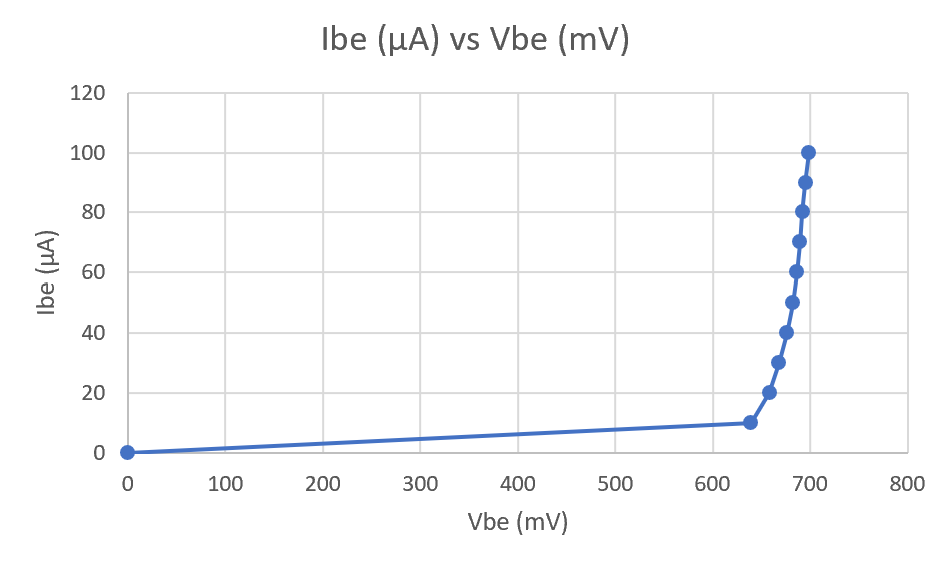
\includegraphics[width=\textwidth]{ECE2200L_Lab5_IV_part1.png}
  \caption{I$_B$ vs V$_{BE}$ chart of 1N2222 at circuit without \SI{500}{\ohm} resistor at collector}
  \label{fig:IV1}
\end{figure}

\newpage

\begin{table}[htbp]
  \centering
  \caption{I$_C$ and V$_{CE}$ values at circuit with \SI{500}{\ohm} resistor at collector}
    \begin{tabular}{rrrrrrr}
      \toprule
          & \multicolumn{2}{c}{$I_{B}=\SI{20}{\micro\ampere}$} & \multicolumn{2}{c}{$I_{B}=\SI{40}{\micro\ampere}$} & \multicolumn{2}{c}{$I_{B}=\SI{60}{\micro\ampere}$} \\
    \multicolumn{1}{r}{V$_{CE}$} & \multicolumn{1}{r}{V$_{CC}$} & \multicolumn{1}{r}{I$_{C}$} & \multicolumn{1}{r}{V$_{CC}$} & \multicolumn{1}{r}{I$_{C}$} & \multicolumn{1}{r}{V$_{CC}$} & \multicolumn{1}{r}{I$_{C}$} \\
    \midrule
    \SI{1 }{\volt}    & \SI{2.28 }{\volt} & \SI{0.002296}{\ampere} & \SI{3.64 }{\volt} & \SI{0.004736}{\ampere} & \SI{4.97 }{\volt} & \SI{0.007122}{\ampere} \\
    \SI{3 }{\volt}    & \SI{4.31 }{\volt} & \SI{0.002350}{\ampere} & \SI{5.72 }{\volt} & \SI{0.004880}{\ampere} & \SI{7.05 }{\volt} & \SI{0.007266}{\ampere} \\
    \SI{5 }{\volt}    & \SI{6.31 }{\volt} & \SI{0.002350}{\ampere} & \SI{7.83 }{\volt} & \SI{0.005077}{\ampere} & \SI{9.28 }{\volt} & \SI{0.007679}{\ampere} \\
    \SI{7 }{\volt}    & \SI{8.36 }{\volt} & \SI{0.002440}{\ampere} & \SI{9.93 }{\volt} & \SI{0.005257}{\ampere} & \SI{11.43}{\volt} & \SI{0.007948}{\ampere} \\
    \SI{9 }{\volt}    & \SI{10.37}{\volt} & \SI{0.002458}{\ampere} & \SI{11.99}{\volt} & \SI{0.005364}{\ampere} & \SI{13.67}{\volt} & \SI{0.008378}{\ampere} \\
    \SI{11}{\volt}    & \SI{12.4 }{\volt} & \SI{0.002512}{\ampere} & \SI{13.98}{\volt} & \SI{0.005346}{\ampere} & \SI{15.95}{\volt} & \SI{0.008881}{\ampere} \\
    \bottomrule
    \end{tabular}%
  \label{tab:IV2}%
\end{table}%

\begin{figure}[H]
  \centering
  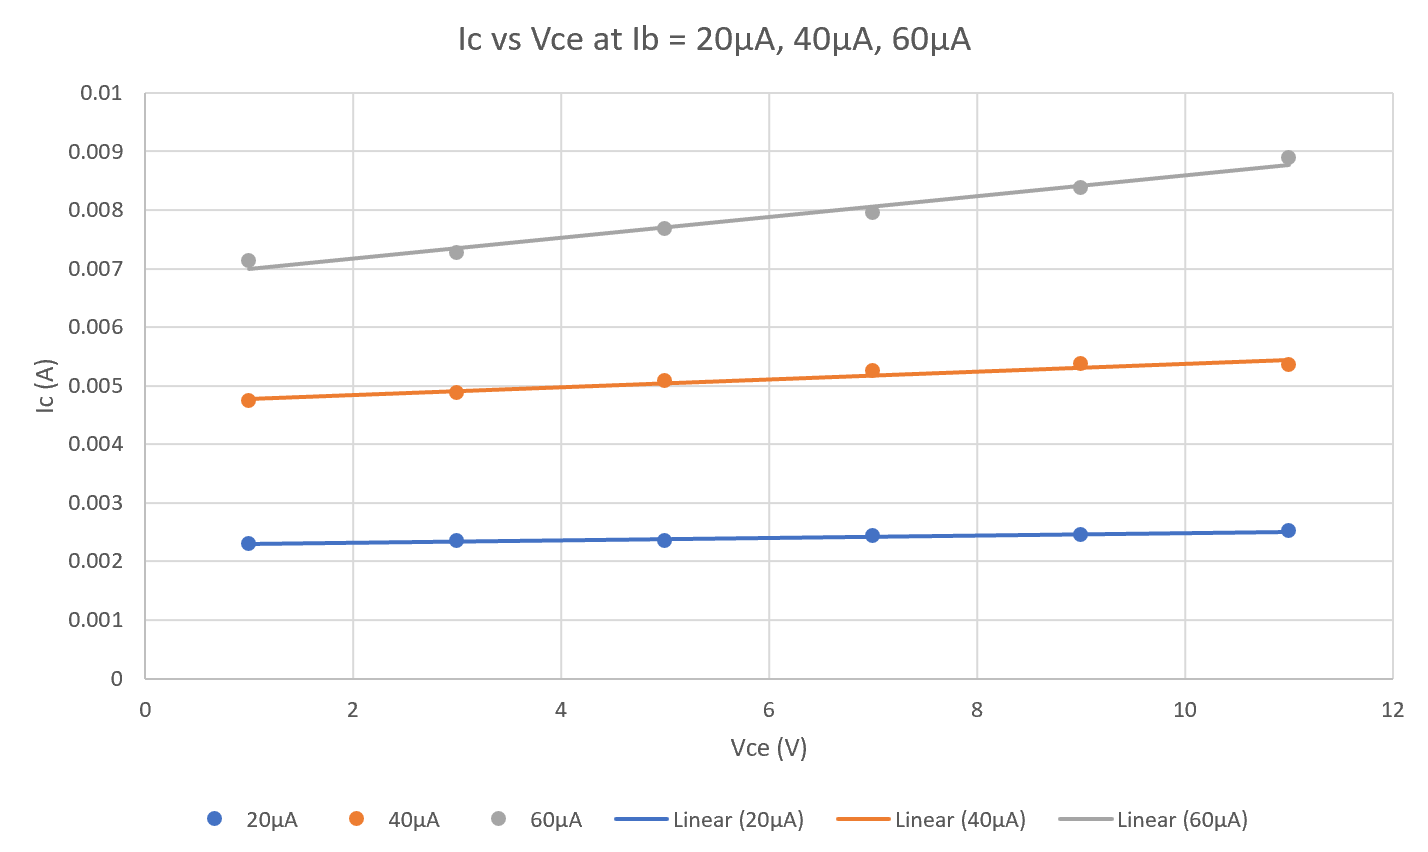
\includegraphics[width=\textwidth]{ECE2200L_Lab5_IV_part2.png}
  \caption{I$_C$ vs V$_{CE}$ chart of 1N2222 at circuit with \SI{500}{\ohm} resistor at collector}
  \label{fig:IV2}
\end{figure}

DC $\beta$ at operating point of $V_{CE} = \SI{5}{\volt}$ and $I_{B} = \SI{40}{\micro\ampere}$ can then be derived.
\begin{equation} \label{eqn1}
  \beta_{DC} = \frac{I_C(V_{CE} = \SI{5}{\volt},I_{B} = \SI{40}{\micro\ampere})}{I_{B} = \SI{40}{\micro\ampere}} = \frac{\SI{0.005077}{\ampere}}{\SI{0.000040}{\ampere}}=126.925
\end{equation} 
\newpage

\begin{figure}[H]
  \centering
  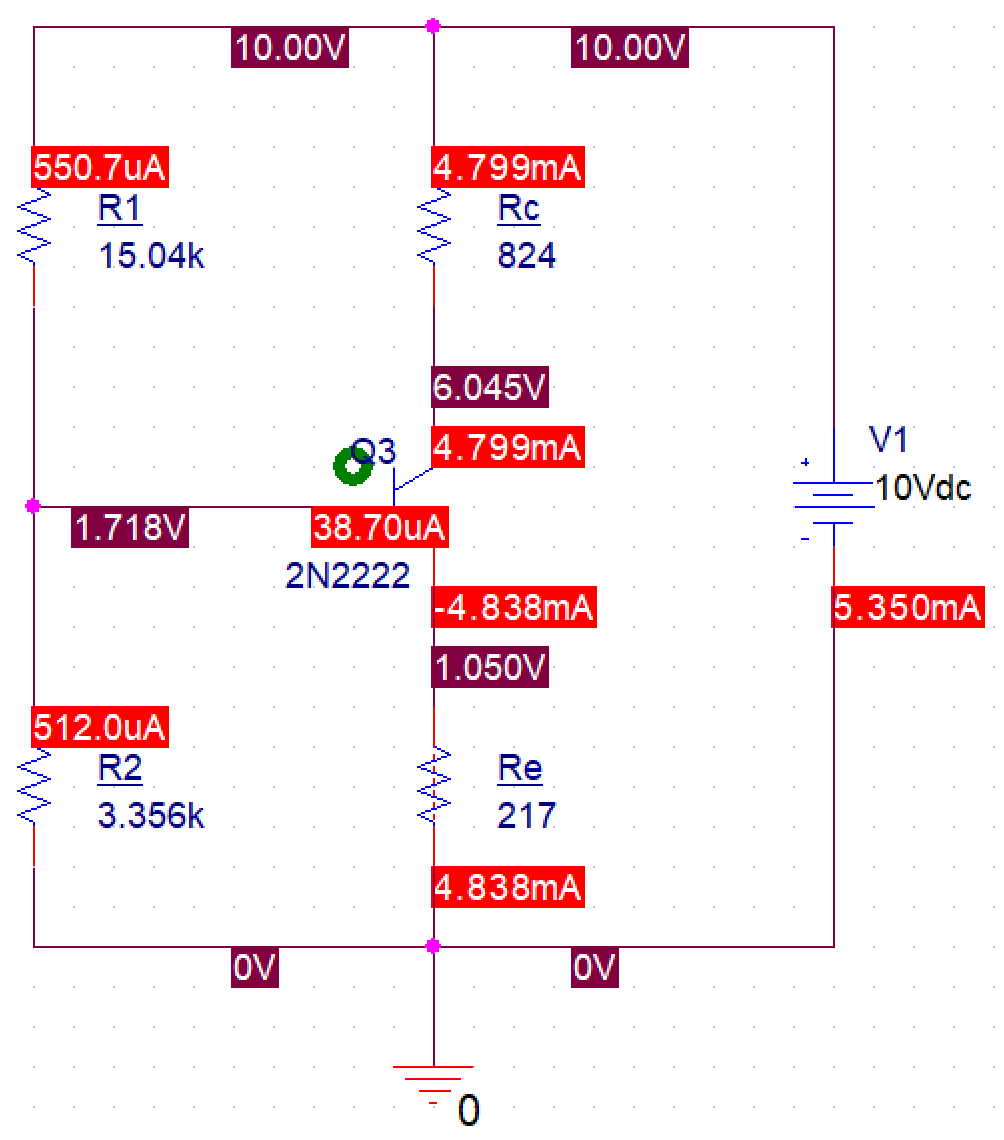
\includegraphics[width=0.9\textwidth]{ECE2200L_Lab5_PSpice.png}
  \caption{PSpice simulation with bias display of the circuit}
  \label{fig:IV2}
\end{figure}

\begin{table}[H]
  \parbox{.45\linewidth}{
  \centering
  \begin{tabular}{rcl}
  $R_1$   &$=$&\SI{15.04}{\kilo\ohm}\\
  $R_2$   &$=$&\SI{3.356}{\kilo\ohm}\\
  $R_E$   &$=$&\SI{217}{\kilo\ohm}\\
  $R_C$   &$=$&\SI{824}{\kilo\ohm}\\
  $V_{CC}$&$=$&\SI{10.00}{\volt}\\
  $V_{C} $&$=$&\SI{5.98}{\volt}\\
  $V_{E} $&$=$&\SI{1.067}{\volt}\\
  $V_{B} $&$=$&\SI{1.719}{\volt}\\
  \end{tabular}
  \caption{Values from circuit}
  \label{tab:valexp}
  }
  \hfill
  \parbox{.45\linewidth}{
  \centering
  \begin{tabular}{ccc}
  $R_1$   &$=$&\SI{15.04}{\kilo\ohm}\\
  $R_2$   &$=$&\SI{3.356}{\kilo\ohm}\\
  $R_E$   &$=$&\SI{217}{\kilo\ohm}\\
  $R_C$   &$=$&\SI{824}{\kilo\ohm}\\
  $V_{CC}$&$=$&\SI{10.00}{\volt}\\
  $V_{C} $&$=$&\SI{6.045}{\volt}\\
  $V_{E} $&$=$&\SI{1.050}{\volt}\\
  $V_{B} $&$=$&\SI{1.718}{\volt}\\  
  \end{tabular}
  \caption{Values from simulation}
  \label{tab:valsim}
  }
  \end{table}

Assuming $I_B$, $I_C$ enter and $I_E$ exit the BJT, for this circuit,
$$ I_C =  \frac{V_{CC}-V_C}{R_C}$$
$$ I_B =  I_E - I_C = \frac{V_E}{R_E}-\frac{V_{CC}-V_C}{R_C}$$
$$ V_{CE} = V_C - V_E $$
$$\beta = \frac{I_C}{I_B}$$

We can then calculate $\beta$ and the BJT bias point $I_B$, $I_C$ and $V_{CE}$ from table \ref{tab:valexp} and table \ref{tab:valsim}.

\begin{table}[H]
  \parbox{.45\linewidth}{
  \centering
  \begin{tabular}{rcl}
  $I_C    $&$=$&\SI{4.88}{\milli\ampere}\\
  $I_B    $&$=$&\SI{38.4}{\micro\ampere}\\
  $V_{CE} $&$=$&\SI{4.913}{\volt}\\
  $\beta  $&$=$&127.1\\
  \end{tabular}
  \caption{Derived from circuit}
  \label{tab:calexp}
  }
  \hfill
  \parbox{.45\linewidth}{
  \centering
  \begin{tabular}{ccc}
    $I_C    $&$=$&\SI{4.799}{\milli\ampere}\\
    $I_B    $&$=$&\SI{38.70}{\micro\ampere}\\
    $V_{CE} $&$=$&\SI{4.995}{\volt}\\
    $\beta  $&$=$&124\\
  \end{tabular}
  \caption{Derived from simulation}
  \label{tab:calsim}
  }
\end{table}


\section*{Conclusion}
From equation \ref{eqn1} we found that $beta = 126.925$, which is close to the value from table \ref{tab:calexp}. The experimental value at table \ref{tab:valexp} and table \ref{tab:calexp} are also similar to the values obtain from PSpice simulation listed in table \ref{tab:valsim} and table \ref{tab:calsim}.

\end{document}
